\documentclass{article}
\usepackage{graphicx}
\usepackage{titlesec}
\usepackage{hyperref}
\usepackage{caption}
\usepackage{listings}
\usepackage{xcolor}
\usepackage[a4paper, margin=1in]{geometry}
\usepackage{float}
\usepackage{tocloft}

% Fix TOC page number alignment
\cftsetindents{subsection}{1.5em}{2.3em}
\setlength{\cftsecnumwidth}{4em}
\setlength{\cftsubsecnumwidth}{5em}

\begin{document}

\begin{titlepage}
    \centering

    % EPITA Logo
    
\includegraphics[width=0.3\textwidth]{figures/Epita.jpg} \\
    \vspace{1cm}

    % Program
    {\large Master in Computer Science} \\
    {\large Software Engineering} \\

    % Main Title
    \vspace{0.5cm}
    {\Huge \textbf{Cloud Computing}} \\
    \vspace{1.3cm}
    {\huge Report 2}
    \vspace{0.1cm}

    % Subtitle
    \vspace{0.5cm}
    {\Large Healthcare Management System Architecture}

    % Team Members
    \vspace{1.5cm}
    {\Large \textbf{Team Members}} \\
    \vspace{0.5cm}
    {\large Jordy Meye} \\
    {\large Huizhe Su} \\
    {\large Arihant Jain} \\
    {\large Nizar} \\

    \vspace{1.5cm}
    {\large March 2026}

\end{titlepage}


\newpage
% --- Styling --- %
\titleformat{\section}
  {\Large\bfseries}
  {Exercise \arabic{section}.}
  {1em}
  {}

\titleformat{\subsection}
  {\normalsize\bfseries}
  {Question \arabic{subsection}.}
  {1em}
  {}

% Code listing style
\lstset{
    basicstyle=\ttfamily\small,
    backgroundcolor=\color{gray!10},
    frame=single,
    breaklines=true,
    postbreak=\mbox{\textcolor{red}{$\hookrightarrow$}\space},
    showstringspaces=false,
    tabsize=4,
    xleftmargin=2em,
    framexleftmargin=1.5em,
}

\raggedbottom
\setlength{\intextsep}{6pt plus 2pt minus 2pt}
\setlength{\floatsep}{6pt plus 2pt minus 2pt}
\setlength{\textfloatsep}{6pt plus 2pt minus 2pt}

\tableofcontents
\newpage

%% ============ SECTION 1: Architecture Overview ============ %%
\section{System Architecture Overview}

\subsection{Objective}

In this lab, we designed a cloud-based Healthcare Management System on AWS. The goal was to build a scalable and secure architecture that can handle patient data, telemedicine, and integrations with existing hospital systems.

The lab required us to cover these areas:
\begin{itemize}
    \item Interoperability with existing hospital systems (HL7/FHIR).
    \item A telemedicine infrastructure for video consultations.
    \item Multi-platform user access.
    \item AI and analytics for clinical decision support.
    \item High scalability and performance.
    \item Cost control.
    \item Security, HIPAA compliance, and disaster recovery.
\end{itemize}
\vspace{14cm}

%% ============ SECTION 2: Architecture Diagram ============ %%
\section{Architecture Design}

\subsection{Visual Representation}

We drew an architecture diagram to map out all the components and how data moves between them. The system is split into layers to keep the frontend, backend, data storage, and security concerns separate.

\begin{figure}[H]
\centering
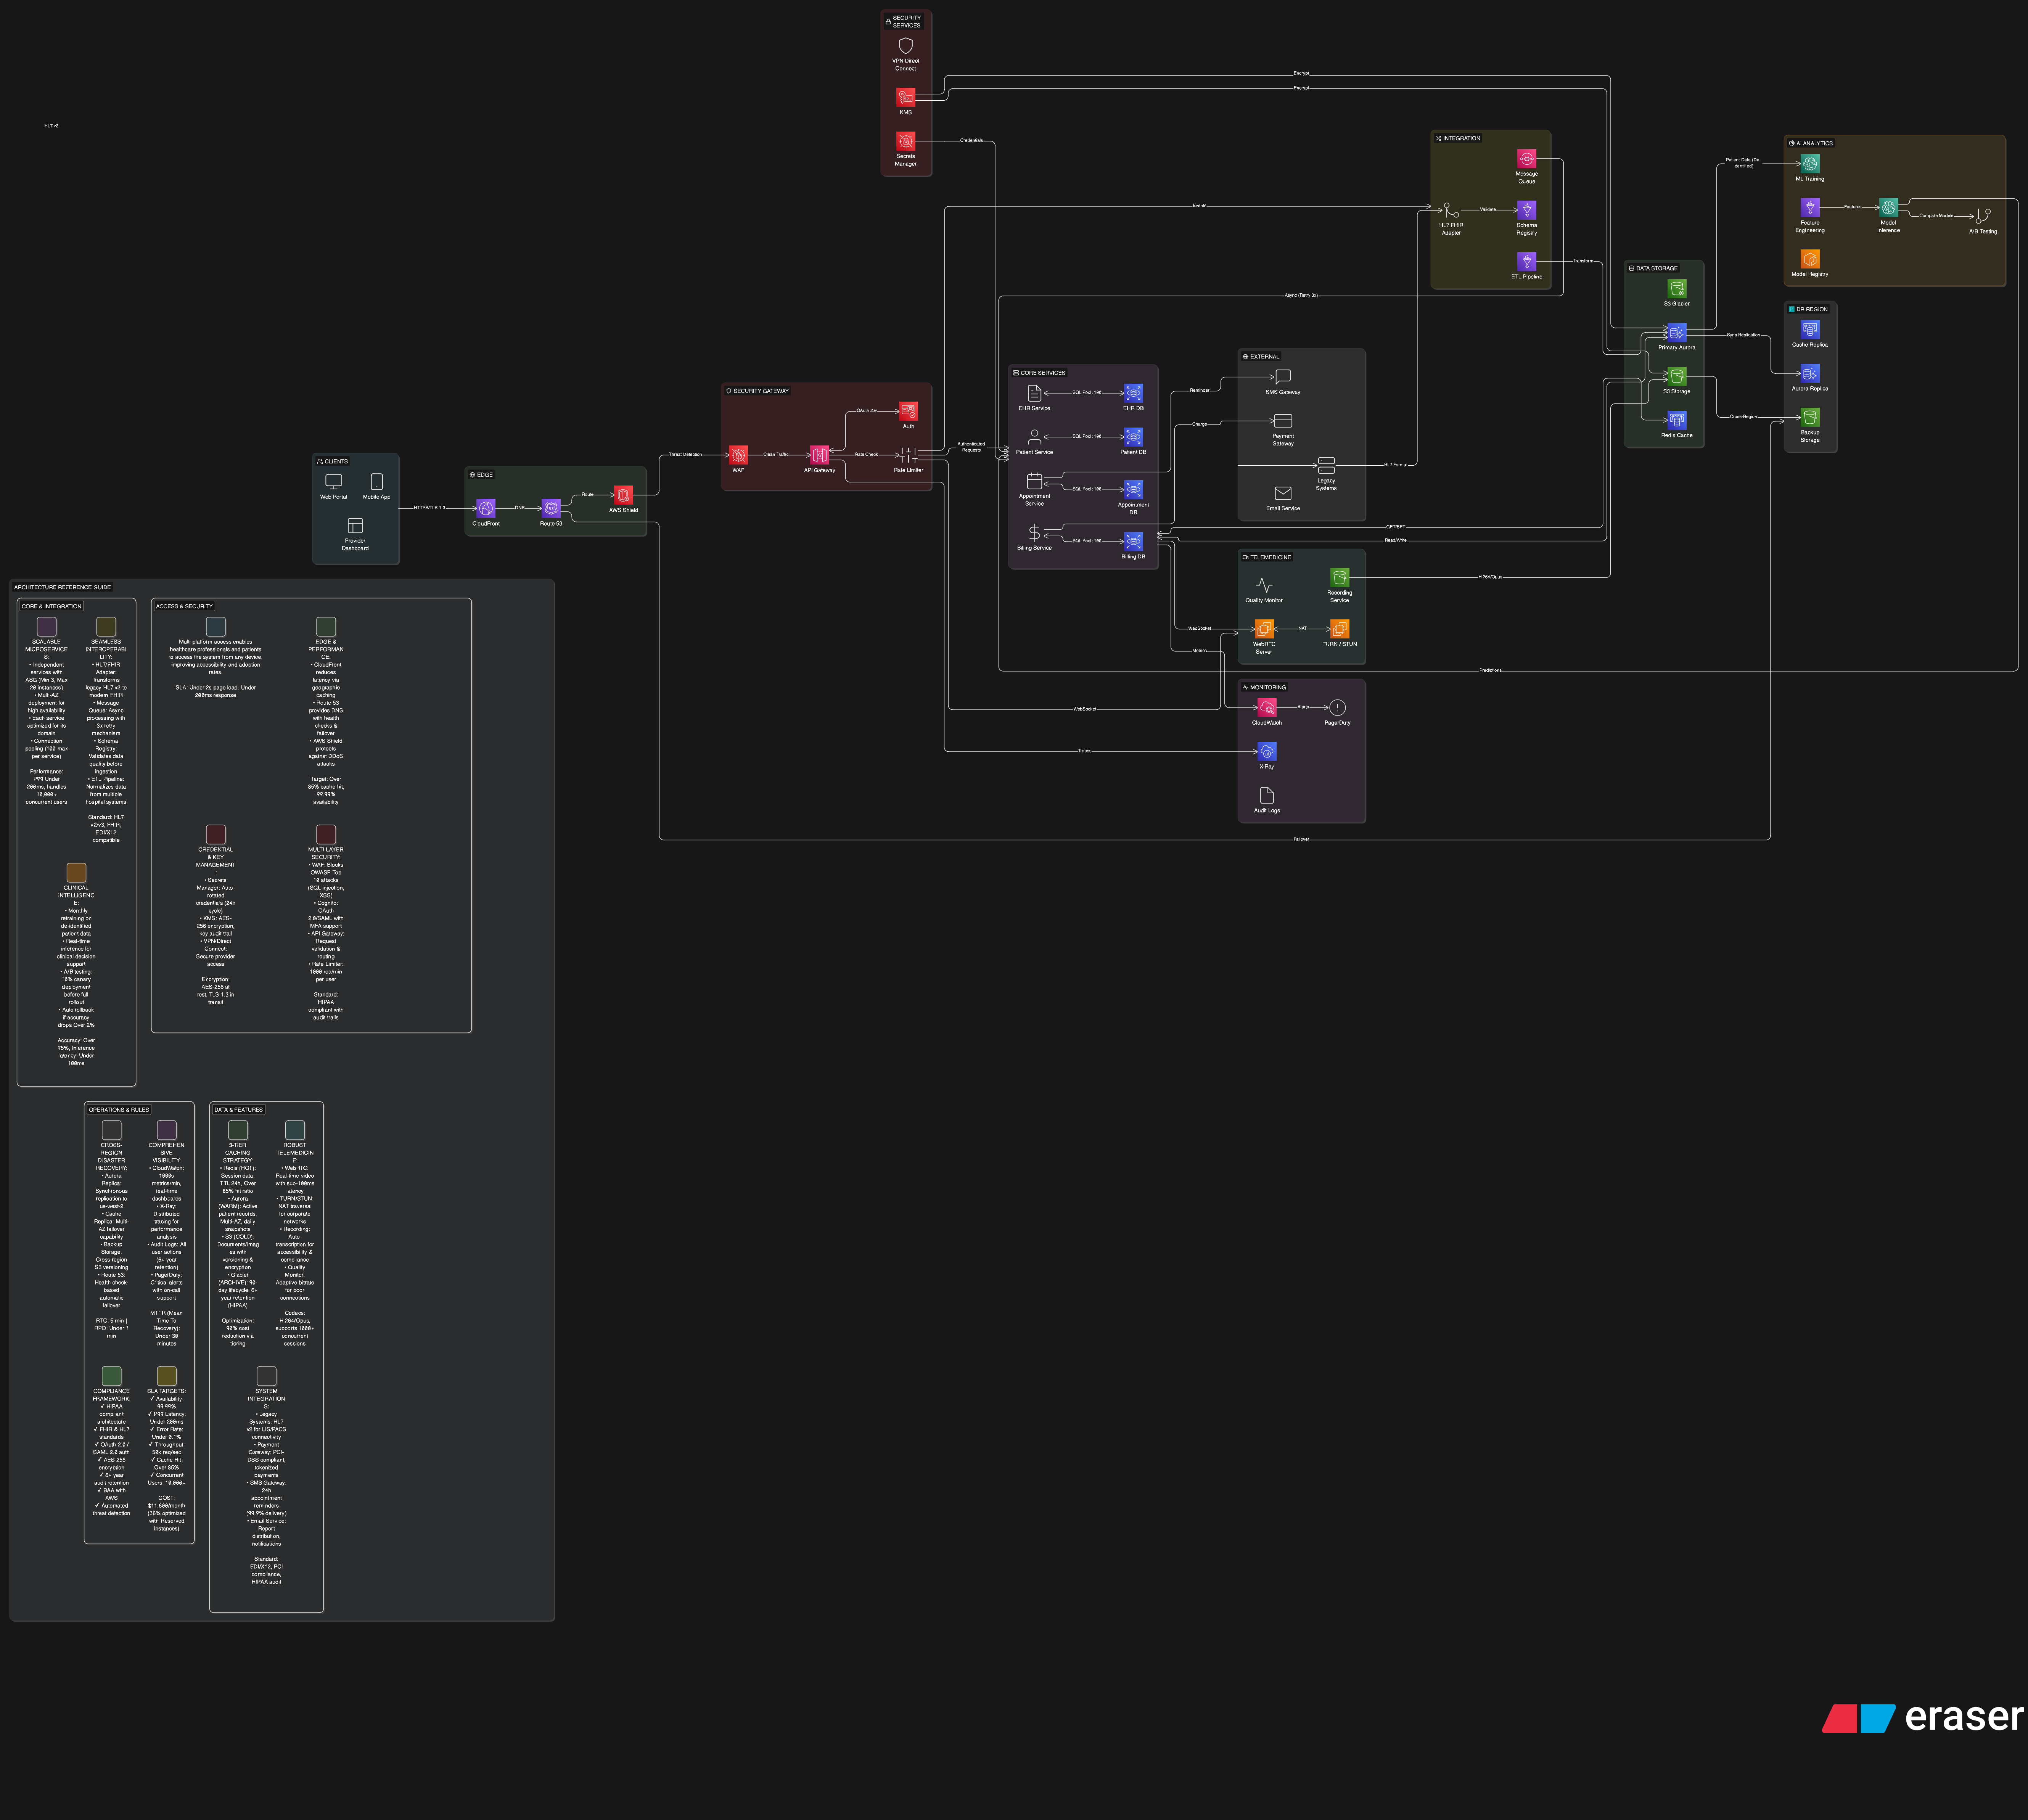
\includegraphics[width=1.0\textwidth]{Healtcare-Architecture-Design-Latest.png}
\caption{Healthcare Management System Architecture}
\end{figure}

The main layers in our design are:
\begin{itemize}
    \item \textbf{Client Layer}: Web portals and mobile apps for patients and providers.
    \item \textbf{Edge \& Security}: CloudFront for caching and AWS WAF to filter incoming web traffic.
    \item \textbf{Core Services}: EC2 instances running microservices for health records, billing, and appointments.
    \item \textbf{Data Storage}: Redis for caching, Aurora for the main database, and S3 for file storage.
    \item \textbf{AI \& Analytics}: SageMaker for machine learning models.
    \item \textbf{Disaster Recovery}: Cross-region replication to a secondary AWS region.
\end{itemize}

%% ============ SECTION 3: Key Components ============ %%
\vspace{8cm}

\section{Detailed Components}

\subsection{Interoperability}
To connect with legacy hospital software, we added an HL7/FHIR adapter at the entry point. Incoming data goes through an AWS Glue schema registry for validation. We also added an SQS queue to buffer messages in case the backend is under load, so nothing gets dropped during a spike.

\subsection{Telemedicine Setup}
For video consultations, we set up a WebRTC server on EC2. We included TURN/STUN servers to handle users behind corporate firewalls. Calls are automatically recorded, the audio is extracted, and the files are saved to S3.

\subsection{Scalability and Performance}
All core microservices are inside Auto Scaling Groups (ASG).
\begin{itemize}
    \item The ASG scales between 3 and 20 instances based on CPU utilization.
    \item An Application Load Balancer distributes the traffic across instances.
    \item We use ElastiCache (Redis) to cache frequent queries and keep API response times under 200ms without hitting the Aurora database every time.
\end{itemize}

\subsection{Data Flow Example}
When a patient registers on the web app, the request goes through the API Gateway, gets authenticated by Cognito, and is saved to the Aurora Patient DB. When they book a telemedicine call, the Appointment Service schedules it and triggers the SMS Gateway to send a reminder. During the call, the WebRTC server handles the video connection. Afterward, the recording goes to S3, and the anonymized text data is pushed to SageMaker to help retrain the clinical AI models.

\subsection{Disaster Recovery (DR)}
We set up the primary region to continuously replicate data to a standby region.
\begin{itemize}
    \item Aurora uses cross-region replication to keep the backup database in sync.
    \item Route 53 health checks monitor the primary region. If it goes down, DNS automatically fails over to the backup.
    \item Our target RTO is 5 minutes.
\end{itemize}

%% ============ SECTION 4: Cost Optimization ============ %%
\vspace{8cm}
\section{Cost Optimization}

To keep AWS costs reasonable, we used a few different strategies:

\begin{enumerate}
    \item \textbf{Reserved Instances}: Databases and base EC2 servers run 24/7, so we plan to use Reserved Instances for them. It gives a significant discount compared to On-Demand pricing.
    \item \textbf{Data Tiering}: We added S3 lifecycle rules. Patient documents and old recordings stay in S3 Standard for 90 days, then get moved to S3 Glacier automatically.
    \item \textbf{Spot Instances}: Monthly ML retraining jobs use Spot Instances since they can tolerate interruptions and don't need to finish immediately.
    \item \textbf{CDN Caching}: Serving static assets through CloudFront reduces data transfer costs from the origin servers.
\end{enumerate}

%% ============ SECTION 5: AI \& Analytics ============ %%
\vspace{4cm}
\section{AI Integration}

We used AWS SageMaker to give doctors clinical decision support. The models can predict disease risks and flag potential drug interactions.

To keep the models accurate, they are retrained monthly using de-identified patient data. When we deploy a new model, we use A/B testing and send only 10\% of traffic to the new version first. If accuracy drops or error rates increase, the system rolls back automatically to the previous model.

%% ============ SECTION 6: Monitoring ============ %%
\vspace{4cm}
\section{System Monitoring}

We set up several monitoring tools to track the health of the system:

\begin{itemize}
    \item \textbf{CloudWatch}: Collects metrics for CPU, memory, and network. We configured alarms to trigger when availability drops below 99.99\%.
    \item \textbf{X-Ray}: Traces requests across the microservices to help find bottlenecks.
    \item \textbf{Audit Logs}: All user actions are logged and stored in S3 for HIPAA compliance.
    \item \textbf{PagerDuty}: Integrated with CloudWatch to alert the on-call team if a critical service goes down.
\end{itemize}

%% ============ SECTION 7: Reflection Questions ============ %%
\vspace{8cm}
\section{Reflection on Proposed Architecture}

\subsection{Scalability Impact}
Using Auto Scaling Groups and a Load Balancer means the system can handle sudden traffic spikes. One thing we thought about was database connection limits during rapid growth. We handled this by adding connection pooling and using Redis to cache reads so not everything goes straight to Aurora.

\subsection{User Accessibility}
We kept the UI flat and simple for users who aren't very technical. The mobile app also includes a voice-to-text feature so patients can describe symptoms without typing. We also added high-contrast mode and large text options.

\subsection{Interoperability Challenges}
The main issue with legacy hospital systems is that HL7 messages can be outdated or badly formatted. We put an AWS Glue schema registry in front of the database to catch these. If a message is invalid, it goes into a dead-letter queue for manual review instead of crashing the pipeline.

\subsection{Telemedicine Ethical Considerations}
All video traffic is encrypted with WebRTC. Recordings are access-controlled and deleted after 90 days. If a patient's connection becomes unstable during a call, the system switches to audio-only automatically to avoid dropping the session entirely.

\subsection{Data Security Measures}
We layered security across the whole stack. AWS WAF sits at the edge to block common exploits. The API Gateway handles rate limiting, and Cognito enforces MFA for all staff accounts. Data is encrypted at rest using KMS (AES-256) and in transit with TLS 1.3.

\subsection{Resource Optimization}
We balanced cost and performance by using S3 lifecycle policies to move old records to Glacier, Reserved Instances for steady workloads, and Spot Instances for background ML training. We will use AWS Cost Explorer to track billing over time.

\subsection{Adaptability to Technological Advancements}
Since we used a microservices architecture, we can update or swap out individual components without touching the rest of the system. For example, adding an IoT patient monitoring service would only require deploying a new microservice. Using the FHIR standard also makes it easier to integrate with future medical APIs.

\subsection{User Training and Support}
The provider dashboard has built-in tooltips. The patient portal has a help section with simple step-by-step guides. We also planned for a ticketing system so users can contact IT support for login or navigation issues.

\subsection{AI Decision Transparency}
The interface shows doctors a confidence score and a reason for each AI prediction. To reduce bias, we made sure the training data includes diverse demographics and we test models against different groups before pushing to production.

\subsection{Disaster Recovery and Contingency Planning}
We rely on a Multi-AZ deployment with a secondary AWS region as the backup. Aurora continuously syncs to the backup region. If the primary region goes down, Route 53 health checks trigger an automatic failover. We also run periodic drills to confirm the recovery time stays under 5 minutes.

%% ============ SECTION 8: Conclusion ============ %%
\section{Conclusion}

In this lab, we designed a cloud architecture for a Healthcare Management System using AWS. The system covers all the requirements from the lab: interoperability with legacy systems, telemedicine support, HIPAA compliance, and cost optimization through data tiering and instance reservations. Using managed services kept the operational overhead low while still giving us the flexibility to scale.

\end{document}